\documentclass{beamer}

\usepackage[utf8]{inputenc}
\usepackage{hyperref}
\usepackage{lmodern}
\usefonttheme{professionalfonts}
\usepackage{amssymb, amsmath}
\usepackage [lambda,
advantage,
operators,
sets,
adversary,
landau,
probability,
notions,
logic,
ff,
mm,
primitives,
events,
complexity,
asymptotics,
keys]{ cryptocode }

\usepackage{tikz}
\usetikzlibrary{arrows}


%Information to be included in the title page:
\title{Lossy Trapdoor Functions}
\author{Giacomo Fenzi}
\institute{ETH Zurich}
\date{22 April 2021}



\begin{document}

\frame{\titlepage}

\begin{frame}
    \frametitle{Motivation}
    \begin{itemize}
        \item Trapdoor Functions are basic primitive, but hard to instantiate
        \item CCA Security from factoring and discrete log but not lattices
    \end{itemize}


\end{frame}


\begin{frame}
    \frametitle{Results}
    \begin{itemize}
        \item Introduce Lossy Trapdoor Functions (LTDFs)
        \item Realize LTDFs from factoring, discrete log \textit{and} lattices
        \item Show LDTFs imply TDFs
        \item Black box construction of CCA-secure (witness recovering) cryptosystems,
              collision-resistant hash functions and oblivious transfer protocols.
    \end{itemize}

\end{frame}

\begin{frame}
    \frametitle{Connections}
    \begin{center}
        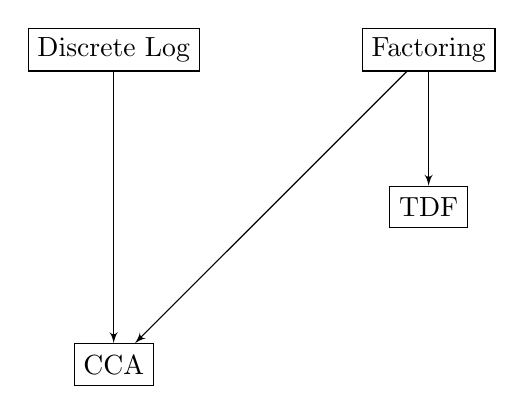
\begin{tikzpicture}
            \tikzset{vertex/.style = {shape=rectangle,draw,minimum size=1.5em}}
            \tikzset{edge/.style = {->,> = latex'}}
            \node[vertex] (a) at  (0,0) {Discrete Log};
            \node[vertex] (b) at  (4,0) {Factoring};
            \node[vertex] (c) at  (0, -4) {CCA};
            \node[vertex] (d) at  (4, -2) {TDF};

            \draw[edge] (b) to (d);
            \draw[edge] (b) to (c);
            \draw[edge] (a) to (c);
        \end{tikzpicture}
    \end{center}
\end{frame}


\begin{frame}
    \frametitle{Connections}
    \begin{center}
        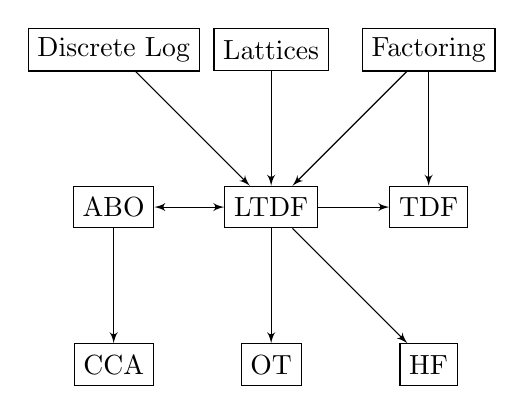
\begin{tikzpicture}
            \tikzset{vertex/.style = {shape=rectangle,draw,minimum size=1.5em}}
            \tikzset{edge/.style = {->,> = latex'}}
            \node[vertex] (a) at  (0,0) {Discrete Log};
            \node[vertex] (j) at  (2,0) {Lattices};
            \node[vertex] (b) at  (4,0) {Factoring};
            \node[vertex] (c) at  (0, -4) {CCA};
            \node[vertex] (d) at  (4, -2) {TDF};
            \node[vertex] (e) at  (2, -2) {LTDF};
            \node[vertex] (f) at  (0, -2) {ABO};
            \node[vertex] (g) at  (2, -4) {OT};
            \node[vertex] (h) at  (4, -4) {HF};

            \draw[edge] (b) to (d);
            \draw[edge] (b) to (e);
            \draw[edge] (a) to (e);
            \draw[edge] (f) to (c);
            \draw[edge] (e) to (d);
            \draw[edge, <->] (e) to (f);
            \draw[edge] (e) to (g);
            \draw[edge] (e) to (h);
            \draw[edge] (j) to (e);
        \end{tikzpicture}
    \end{center}
\end{frame}

\begin{frame}
    \frametitle{Notation and Entropy}
    \begin{itemize}
        \item $\secpar$ is the security parameter, and
              we will abbreviate $n(\secpar) = \poly$ as simply $n$
        \item $f({-})$ denotes the function taking $x \mapsto f(x)$
        \item Write $H_\infty(X)$ for the min-entropy of $X$. This corresponds to the optimal probability of guessing $X$.
        \item We let $\widetilde{H}_\infty(X|Y)$ be the average min-entropy of $X$ conditioned on $Y$.
              This corresponds to the optimal probability of guessing $X$ knowing $Y$.
        \item We use the following lemma, if $Y$ takes at most $2^r$ values then:
              \[ \widetilde{H}_\infty(X|Y) \geq H_\infty(X) - r \]
    \end{itemize}
\end{frame}

\begin{frame}
    \frametitle{Trapdoor Functions}
    Informally, a trapdoor function is family of functions that are
    hard to invert without access to some additional information called a trapdoor
    \begin{definition}
        A trapdoor function consists of three PPT algorithms $(S, F, F^{-1})$
        such that:
        \begin{itemize}
            \item \textit{Easy to sample and invert with trapdoor.} $S(\secparam) \rightarrow (s, t)$
                  such that $F(s, {-})$ is an injective function on $\bin^n$ and $F^{-1}(t, {-})$ is its inverse
            \item \textit{Hard to invert without.} For \textit{any} PPT inverter $\adv$ we have that $\adv(\secparam, s, F(s, x))$
                  outputs $x$ with negligible probability.
        \end{itemize}
    \end{definition}
\end{frame}

\begin{frame}
    \frametitle{Example of Trapdoor}
    RSA Encryption! In trapdoor form:
    \begin{itemize}
        \item $S(\secparam)$ generates $N, e, d$ as in RSA,
              set $s \coloneqq (N, e)$ and $t \coloneqq (d)$ and returns $(s, t)$
        \item $F(s, x)$ computes $x^e \mod N$
        \item $F^{-1}(t, c)$ computes $c^d \mod N$
    \end{itemize}
    Composite Residuosity
    \begin{itemize}
        \item $S(\secparam)$ generates $N = pq$ as a product of large primes,
              select $g$ suitably, $s \coloneqq (N, g)$, $t \coloneqq (p, q)$
        \item $F(s, x)$ splits $x = m_1 + N m_2$ and returns $g^{m_1} m_2^N \mod N^2$
        \item $F^{-1}(t, c)$ decrypts using the factorization to compute Carmichael function
    \end{itemize}
\end{frame}

\begin{frame}
    \frametitle{Lossy Trapdoors}
    Informally, you either get an injective trapdoor or a 'lossy' function, and \textit{cannot tell which is which}
    \begin{definition}
        A ($n$, $k$)-lossy trapdoor function consists of three PPT algorithms $(S, F, F^{-1})$.
        We denote $S_{inj}({-}) \triangleq S({-}, 0)$ and $S_{lossy}({-}) \triangleq S({-}, 1)$.
        \begin{itemize}
            \item \textit{Outputs of $S_{inj}$ are easy to compute and easy to invert with trapdoor.}
                  $S_{inj}(\secparam) \rightarrow (s, t)$ s.t. that $F(s, {-})$, $F^{-1}(t, {-})$ are in the trapdoor case
            \item \textit{Outputs of $S_{lossy}$ are easy to compute}.
                  $S_{lossy}(\secparam) \rightarrow (s, \bot)$ s.t. $F(s, {-})$ is a function on $\bin^n$
                  with image size at most $2^{n-k}$.
            \item The first outputs of $S_{inj}(\secparam)$ and $S_{lossy}(\secparam)$ are computationally indistinguishable.
        \end{itemize}
    \end{definition}
\end{frame}

\begin{frame}
    \frametitle{Subleties}
    \begin{itemize}
        \item The definition really relates to a collection of lossy trapdoor functions.
        \item $k \triangleq k(\secpar) = \poly \leq n$ is a parameter that represents how 'lossy' the collection is.
        \item We also write $r \triangleq n-k = \poly$ as the \textit{residual leakage}.
        \item No hardness requirement on inverting outputs of $S_{inj}$
        \item Requirements are too strict in lattices, leads to \textit{almost-always} lossy functions.
    \end{itemize}
\end{frame}

\begin{frame}
    \frametitle{All-But-One TDFs}
    Intuition: Most branches\footnote{Subsequent work often calls these tags} are trapdoors, except one which is lossy. You cannot tell which one it is.
    \begin{definition}
        An $(n, k)$-ABO TDF is a triple of PPT algorithms $S, F, F^{-1}$ such that:
        \begin{itemize}
            \item $S(\secparam, b^*) \rightarrow (s, t)$ as before
            \item For any $b \neq b^*$, $F(s, b, {-})$ $F^{-1}(t, b, {-})$ are as in the previous definition.
            \item $F(s, b^*, {-})$ is a lossy function as before
            \item For any $b,b'$ the first outputs of $S(\secparam, b)$, $S(\secparam, b')$ are computationally indistinguishable.
        \end{itemize}
    \end{definition}
\end{frame}

\begin{frame}
    \frametitle{ABO $\equiv$ LTDF}
    \begin{itemize}
        \item ABOs and LTDFs are equivalent.
        \item ABO $\implies$ LTDF. Take ABO on $\bin$ and evaluate always on one of the branches, but switch lossy branch on generation.
        \item LTDF $\implies$ ABO. Generate an ABO on $\bin$ by having $s = (s_0, s_1)$ where one of the two is lossy, and evaluation by using $s_b$
        \item Finally, we can extend ABOs on $\bin$ to ABOs on $\bin^\ell$ at the cost of having residual leakage $\ell r$. The idea is,
              for lossy branch $b^* \in \bin^\ell$, generate $\ell$ ABOs each with the $i$-th having lossy branch $b^*_i$.
    \end{itemize}
\end{frame}

\begin{frame}
    \frametitle{LTDF $\implies$ TDF}
    \begin{itemize}
        \item Completeness: Use the injective functions generated by $S_{inj}$.
        \item Soundness: We cannot (information theoretically) invert the lossy branch,
              so if we could invert the injective trapdoors we could distinguish outputs
              of $S_{inj}, S_{lossy}$, contradicting LDTFness.
        \item Formally, let $\adv$ be an inverter. We build $\ddv$
              \begin{pchstack}[center]
                  \procedure{$\ddv^\adv(s)$}{
                      x \sample \bin^n \\
                      y = F(s, x) \\
                      x' = \adv(s, y) \\
                      \pcreturn x = x'
                  }
              \end{pchstack}
              We analyze this in the next slide
    \end{itemize}
\end{frame}

\begin{frame}
    \frametitle{LTDF $\implies$ TDF}
    Note that if $s$ is generated by $S_{inj}$ then with some non negligible probability
    we have that $\adv$ succeeds and $\ddv$ succeeds whenever $\adv$ does.

    Instead, if $s$ is generated by $S_{lossy}$ even an unbounded adversary
    would have best possible probability given by $2^{-\widetilde{H}_\infty(x|s, F(s, x))}$.
    But note that $F(s, {-})$ takes at most $2^r$ values and so by the previous
    lemma $\widetilde{H}_\infty(x|s, F(s, x)) \geq H_\infty(x|s) - r = n - (n - k) = k$.
    So the probability is bounded by $2^{-k}$ and as such is negligible.

    From the above it follows that $\ddv$ will win the distinguishing game with non negligible probability.

\end{frame}

\begin{frame}
    \frametitle{LTDF $\implies$ CCA}
    \framesubtitle{Requirements}
    We will have some requirements primitives\footnote{All of these reduce to LTDFs}.
    We note that our cryptosystem will have message space $\bin^\ell$.
    \begin{itemize}
        \item We have $\Sigma = (\mathrm{Gen}, \mathrm{Sign}, \mathrm{Vfy})$ a strongly unforgeable one-time signature scheme. We require that the public keys are in $\bin^v$.
        \item $F = (S_{ltdf}, F_{ltdf}, F^{-1}_{ltdf})$ is a $(n, k)$-lossy trapdoor function.
        \item $G = (S_{abo}, F_{abo}, F^{-1}_{abo})$ is a $(n, k')$-ABO trapdoor function with branch space $\bin^v$.
        \item $\mathcal{H}$ is a collection of pairwise independent hash functions $\bin^n \to \bin^\ell$.
        \item We require that $k + k' \geq n + \kappa$ for some $\kappa = \omega(\log n)$ and that $\ell \leq \kappa - 2 \lg(1/\epsilon)$ from $\epsilon = \negl$
    \end{itemize}
\end{frame}

\begin{frame}
    \frametitle{LTDF $\implies$ CCA}
    \framesubtitle{Encryption Scheme}

    \begin{pchstack}
        \procedure{$\mathcal{G}(\secparam)$}{
            (s, t) \leftarrow S_{inj}(\secparam) \\
            (s', t') \leftarrow S_{abo}(\secparam, 0^v) \\
            h \sample \mathcal{H} \\
            pk \coloneqq (s, s', h) \\
            sk \coloneqq (t, t', pk) \\
            \pcreturn (pk, sk)
        }


        \procedure{$\mathcal{E}(pk, m)$}{
        (vk, sk_\sigma) = \mathrm{Gen}(\secparam) \\
        x \sample \bin^n \\
        c_1 = F_{ltdf}(s, x) \\
        c_2 = G_{abo}(s, vk, x) \\
        c_3 = m \xor h(x) \\
        \omega \leftarrow \mathrm{Sign}(sk_\sigma, (c_i)_{i=1}^3) \\
        \pcreturn (vk, c_1, c_2, c_3, \sigma)
        }


        \procedure[space=auto]{$\mathcal{D}(sk, c)$}{
        \pcif \neg \mathrm{Vfy}(vk, (c_i)_{i = 1}^3, \sigma) \\
        \pcreturn \bot \\
        \pcfi \\
        x = F^{-1}(t, c_1) \\
        \pcif c_1 \neq F_{ltdf}(s, x) \, \vee \\
        c_2 \neq G_{abo}(s, vk, x) \\
        \pcreturn \bot \\
        \pcfi \\
        \pcreturn c_3 \xor h(x)
        }
    \end{pchstack}

\end{frame}

\begin{frame}
    \frametitle{LTDF $\implies$ CCA}
    \framesubtitle{CCA Game}
    Correctness is easy to check. We next show security in the single
    encryption CCA security game. Below we show the formal game definition.
    $\mathrm{Setup}$ is to be called once at the beginning of the game, and
    the attacker is allowed a single query to $\mathrm{EncO}$ and oracle access to
    $\mathrm{DecO}$. The attacker wins if it outputs $b' = b$.
    \begin{center}
        \begin{pchstack}
            \procedure{$\mathrm{Setup}(\secpar)$}{
                b \sample \bin \\
                \mathcal{T}_{enc} = \emptyset \\
                pk, sk \leftarrow \mathcal{G}(\secpar) \\
                \pcreturn pk
            }
            \procedure{$\mathrm{EncO}(m_0, m_1)$}{
                c \leftarrow \mathcal{E}(pk, m_b) \\
                \mathcal{T}_{enc} \coloneqq \mathcal{T}_{enc} \cup \set{c} \\
                \pcreturn c
            }
            \procedure{$\mathrm{DecO}(c^*)$}{
                \pcif c^* \in \mathcal{T}_{enc} \\
                \t \pcreturn \bot \\
                \pcfi \\
                \pcreturn \mathcal{D}(sk, c^*)
            }
        \end{pchstack}
    \end{center}

\end{frame}

\begin{frame}
    \frametitle{LTDF $\implies$ CCA}
    \framesubtitle{Game Hops}
    We proceed by a sequence of games. We note that, since a single query
    is made to $\mathrm{EncO}$ we move the signature scheme generation in
    $\mathrm{Setup}$ and denote that verification key as $vk^*$.
    \begin{gamedescription}[name=G]
        \describegame This is the original CCA Security Game
        \describegame In $\mathrm{DecO}$ if $vk=vk^*$ return $\bot$
        \describegame In $\mathrm{Setup}$ choose the lossy branch of $G$ to be $vk^*$
        \describegame In $\mathrm{DecO}$ find $x$ using $G$'s trapdoor rather than $F$'s
        \describegame In $\mathrm{Setup}$ replace $S_{inj}$ with $S_{lossy}$
    \end{gamedescription}
    The hops are as follows:
    \[ G_1 \approx_\Sigma G_2\approx_{abo} G_3 \equiv G_4 \approx_{ltdf} G_5 \]
    Finally, an argument as in TDF case shows that in $G_5$ even an unbounded attacker has only
    negligible success probability.
\end{frame}
\begin{frame}
    \frametitle{Realizations}
    We can realize LTDF from \textit{any} encryption scheme that is:
    \begin{itemize}
        \item Additively Homomorphic. This allows to encrypt either $\mathbf{I}_n$ or $\mathbf{0}_n$ indistinguishably and to
              evaluate at $\mathbf{x}$ by computing $\mathbf{xM}$.
        \item Secure to Reuse Randomness, so that we can use the same randomness with different keys securely.
        \item Isolated Randomness, so that it is only dependent on the input randomness and not on keys/messages.
    \end{itemize}
    We shows next a realization from the DDH assumption, but a similar technique
    can also be employed with lattices (based on $\mathrm{LWE}$) with some difficulties.
\end{frame}
\begin{frame}
    \frametitle{DDH $\implies$ LTDF}
    Consider the following variant of the ElGamal cryptosystem, with public key $h = g^z$ and secret key $z$.
    The encryption function is $E_h(m; r) = (g^r, h^r g^m)$ for randomness $r$. To decrypt $(c_1, c_2)$
    we output $\log_g(c_2/c_1^z)$ which is easy to compute if $m \in \bin$.

    This scheme is semantically secure and it is additively\footnote{All operations done component wise} homomorphic i.e.
    \[ E_h(m; r) \odot E_h(m'; r') = E_h(m + m', r + r')\]
    \[ E_h(m; r)^x = E_h(mx; rx) \]
\end{frame}

\begin{frame}
    \frametitle{DDH $\implies$ LTDF}
    We show how to use the previous scheme to encrypt a matrix $\mathbf{M} = (m_{i, j}) \in \ZZ_p^{n \times n}$.
    Select $n$ pk/sk pairs $h_i = g^{z_i}$ and $n$ pieces of randomness $r_i$.
    Then the encryption is the matrix $\mathbf{C} = (c_{i,j}) = (E_{h_j}(m_{i,j}; r_i))$ with the $z_j$s as decryption keys.

    We can represent $\mathbf{C}$ as the following two matrices:
    \[ \mathbf{C_1} = \begin{bmatrix}
            g^{r_1} \\
            \vdots  \\
            g^{r_n}
        \end{bmatrix}, \;
        \mathbf{C_2} = \begin{bmatrix}
            h_1^{r_1} g^{m_{1,1}}  & \dots  & h_n^{r_1} g^{m_{1,n}}  \\
            \vdots                 & \ddots & \vdots                 \\
            h_1^{r_n} g^{m_{n, 1}} & \dots  & h_n^{r_n} g^{m_{n, n}}
        \end{bmatrix}\]
    Via $n^2$ hybrid games we can show that this encryption produces indistinguishable
    ciphertext under DDH. We denote this operation as $\mathrm{ME}(\mathbf{z}, \mathbf{M})$ for
    $\mathbf{z}$ the vector of private keys.
\end{frame}

\begin{frame}
    \frametitle{DDH $\implies$ LTDF}
    We build a LTDF from the previous scheme as it follows. Note
    that in the injective case we encrypt the identity matrix, while
    in the lossy the all zero matrix.
    \begin{center}
        \begin{pchstack}
            \procedure{$S_{inj}(\secparam)$}{
                \mathbb{G} \leftarrow \mathcal{G}(\secparam) \\
                \mathbf{z} \sample \ZZ^n_p \\
                \mathbf{C} \leftarrow \mathrm{ME}(\mathbf{z}, \mathbf{I}_n) \\
                \pcreturn (\mathbf{C}, \mathbf{z})
            }
            \procedure{$S_{lossy}(\secparam)$}{
                \mathbb{G} \leftarrow \mathcal{G}(\secparam) \\
                \mathbf{z} \sample \ZZ^n_p \\
                \mathbf{C} \leftarrow \mathrm{ME}(\mathbf{z}, \mathbf{0}_n) \\
                \pcreturn (\mathbf{C}, \bot)
            }
            \begin{pcvstack}
                \procedure{$F_{ltdf}(\mathbf{C}, \mathbf{x})$}{
                    \pcreturn \mathbf{y} = \mathbf{x} \mathbf{C}
                }

                \pcvspace

                \procedure{$F^{-1}_{ltdf}(\mathbf{z}, \mathbf{y})$}{
                    x_i = D_{z_i}(y_i) \\
                    \pcreturn \mathbf{x}
                }
            \end{pcvstack}
        \end{pchstack}
    \end{center}
\end{frame}
\begin{frame}
    \frametitle{DDH $\implies$ LTDF}
    \framesubtitle{Subleties}
    \begin{itemize}
        \item $\mathcal{G}$ is the group generation algorithms, it returns $(G, p, g)$ where
              $G$ is a cyclic group of prime order $p$ with generator $g$. We assume DDH hardness w.r.t. $\mathcal{G}$.
        \item $\mathbf{xC}$ is computed by the homomorphic property.
              In fact, if $\mathbf{C} = \mathrm{ME}(\mathbf{z}, \mathbf{M})$ with randomness $\mathbf{r}$ and $h_j = g^{z_j}$
              \[ y_j = \bigodot_{i=1}^n c_{i,j}^{x_i} = E_{h_j}((\mathbf{xM})_j ; R \triangleq \langle \mathbf{r}, \mathbf{x} \rangle) \]

        \item Note that if $\mathbf{M} = \mathbf{I}_n$ then $y_j = E_{h_j}(x_j; R)$
        \item If instead $\mathbf{M} = \mathbf{0}_n$ then $y_j = E_{h_j}(0; R)$
    \end{itemize}
\end{frame}
\begin{frame}
    \frametitle{DDH $\implies$ LTDF}
    \framesubtitle{Final Checks}
    Now, we just have to check that the LTDF conditions are satisfied.
    In particular, the above construction is $(n, n - \lg p)$-lossy.
    \begin{itemize}
        \item The three algorithms are clearly PPT
        \item A quick thought shows that the injective conditions are met
        \item Indistinguishability follows from the indistinguishability of $\mathrm{ME}$.
        \item Finally, for outputs generated by $S_{loss}$ we have that
              $y_i = E_{h_i}(0; R)$ for some $R \in \ZZ_p$ that depends on $x$. $R$ can take
              at most $p$ values, the residual leakage is at most $\lg p$ and so the loss is
              $k = n - r \geq n - \lg p$
    \end{itemize}
\end{frame}

\begin{frame}
    \frametitle{Things which I did not have time to show}
    \begin{itemize}
        \item More efficient ABO construction from DDH
        \item LDTFs from LWE
        \item CPA from LTDFs
        \item SUF one time signatures from LDTFs
        \item UOWHFs, CRHFs from LDTFs
        \item OT from LDFTs
    \end{itemize}
\end{frame}

\begin{frame}
    \frametitle{Related Work}
    \begin{itemize}
        \item All-But-Many LTDFs
        \item Identity Based LTDFs
    \end{itemize}
\end{frame}

\end{document}